
\section{实施得分中心化}
\label{sec:sc_implementation}

\begin{notationbox}
\textbf{符号}（如 \Cref{sec:sc} 所示）。在固定前缀下，$y_t$ 为采样得到的 token，$v$ 为词表中的 token；$p_v$、$q_v$ 分别为其训练器和采样器的概率，$s_v = \nabla_\theta \log p_v$ 为其得分，$\bar{s} = \sum_v q_v \, s_v$ 为采样器下的期望得分。
\end{notationbox}

\subsection{Top-$k$ 近似}

\textit{完整} 得分中心化，如我们迄今所描述的，对大多数实际应用而言成本过高。按照 \Cref{eq:sc} 所述，计算得分中心化校正项（即对采样器每个 token 分布的得分期望）需要存储每个采样 token 的完整输出 logprobs。例如，Qwen3 模型的词表大小为 152K，仅以 fp32 精度存储单个 token 的完整 logprobs 就需要约 608KB 内存。假设批量为 1024 次回溯，每条序列长度为 32K，存储完整 logprobs 将需要高达 20TB 的内存。因此，我们在实验中仅存储采样器分布的 top-$k$ 近似，其中 $k=128$ 。然而，我们并未仅仅在 top-$k$ 分布上计算期望得分，而是仍尝试通过训练器提供的 logprobs 来填补尾部，以近似采样器的完整分布。我们采用 $k=128$ 作为保守默认值；\Cref{fig:top_k} 表明，$k=128$ 甚至 $k=32$ 在所有实验情景下均与完整得分中心化表现相当。

问题是如何仅从采样器的前-$k$ 个最高对数概率中重构其完整的分布。  
设 $\hat{q}$  表示我们对采样分布的近似。  
我们取采样器的前-$k$ 个最高对数概率，并使用训练器提供的对数概率来建模尾部，经过缩放使得整个分布的总和为一。记前-$k$ 个 token 组成的集合为头部 $H$ ，其余 token 组成的集合为尾部 $T$ ：
\begin{equation}
\hat{q}_v =
\begin{cases}
q_v & v \in H \\[2pt]
\rho \, p_v & v \in T
\end{cases}
\qquad \textrm{where} \quad
\rho = \frac{1 - \sum_{v \in H} q_v}{1 - \sum_{v \in H} p_v}.
\label{eq:tail_model}
\end{equation}
标量 $\rho$  是采样器尾部质量与训练器尾部质量的比值——它对训练器的尾部进行缩放，使得 $\hat{q}$  的和为一。

为在该重构的 $\hat{q}$ 分布下计算期望得分，无需对整个词表求和。相反，我们确切地计算从 $q$ 中取出的头部的期望值，并利用“全词表上的期望得分之和为零”这一性质，将从 $p$ 中取出的尾部的期望值计算为零减去头部的期望值：
\begin{equation}
\mathbb{E}_{\hat{q}}[s_{y_t}]
= \sum_{v \in H} q_v \, s_v + \rho \sum_{v \in T} p_v \, s_v
= \sum_{v \in H} q_v \, s_v + \rho \, \Big( \underbrace{\mathbb{E}_p[s_{y_t}]}_{=\,0} - \sum_{v \in H} p_v \, s_v \Big)
= \sum_{v \in H} \left( q_v - \rho \, p_v \right) s_v.
\label{eq:sc_topk}
\end{equation}
因此，居中项仅涉及 $k$ 头 token，尽管建模的尾部覆盖了整个词表。

top-$k$  得分中心的开销可忽略不计：在匹配的硬件上，$k=128$  的运行时间与基准方法相比，在 0.6B 和 30B 模型上均不超过 1\% 的时钟时间。我们的自定义 JAX 采样器在解码过程中计算 top-$k$  对数概率；vLLM 和 SGLang 原生支持 top-$k$  对数概率，但我们尚未测量其开销。

\subsection{组合得分中心化与重要性采样}
\label{sec:is_composition}

得分中心化通过减去一个等于期望得分的修正项来实现。重要性采样方法如TIS或MIS通过使用截断/掩码的重要度比率对得分进行重新加权。因此，当在重要性采样之上组合得分中心化时，我们计算的是\textit{加权}得分的期望值，而非原始得分的期望值。我们可以将其理解为：首先通过IS对得分进行重新加权，然后在重新加权后的得分上应用得分中心化。

\clearpage
令 $r_v = p_v / q_v$ 表示重要性比率，$w_v = f(r_v)$ 表示由 IS 方法分配的权重，例如 $f(r) = \min(r, 2)$ 表示 TIS。得分中心化减去 \textit{加权} 得分的期望：
\begin{equation}
R \left( w_{y_t} \, s_{y_t} - \mathbb{E}_q[w_{y_t} \, s_{y_t}] \right),
\qquad
\mathbb{E}_q[w_{y_t} \, s_{y_t}] = \sum_v q_v \, w_v \, s_v.
\label{eq:sc_is}
\end{equation}
与普通的得分中心化类似，当奖励为常数时，期望更新恰好为零——通过减去期望加权得分 $\mathbb{E}_q[w_{y_t} \, s_{y_t}]$，根据构造可消除漂移，无论权重函数 $f(r)$ 如何。

顶部-$k$ 约简在 \Cref{eq:sc_topk} 中同样适用。在建模的尾部，采样器概率仅通过 $\hat{q}$ 得知，因此权重也在 $\hat{q}$ 下计算：$\hat{w}_v = f(p_v / \hat{q}_v)$，该式在头部等于 $w_v$。由于 $p_v / \hat{q}_v = p_v / (\rho \, p_v) = 1/\rho$ 在尾部为常数，中心化项保持相同的仅头部形式，其中用标量 $\alpha$ 替代了 $\rho$：
\begin{equation}
\mathbb{E}_{\hat{q}}[\hat{w}_{y_t} \, s_{y_t}] = \sum_{v \in H} \left( q_v \, w_v - \alpha \, p_v \right) s_v,
\qquad \textrm{where} \quad
\alpha = \rho \, f(1/\rho).
\label{eq:sc_is_topk}
\end{equation}
Vanilla 得分中心化只是 $f = 1$ 的一个特例，给出 $\alpha = \rho$。作为合理性检查，Vanilla 重要性采样 $f(r) = r$ 给出 $\alpha = 1$ 和 $q_v \, w_v = p_v$，因此中心化项消失——确切的重要性采样已经具有零期望加权得分，所以无需再进行中心化。

\subsection{损失公式}

得分中心化可以通过在自动生成梯度框架中将其实现到标量损失函数内来高效实现。由于期望得分是每个 token 得分的加权和，$\bar{s} = \sum_v q_v \, \nabla_\theta \log p_v$，我们可以将得分中心化表示为一个损失，通过使用分离的采样器概率对训练者的对数概率进行加权。对于策略梯度，这变为：
\begin{equation}
L = -R \, \Big( \log p_{y_t} - \underbrace{\sum_v \operatorname{sg}\left[ q_v \right] \log p_v}_{\text{centering term}} \Big),
\label{eq:sc_loss}
\end{equation}
其中 $\operatorname{sg}[\cdot]$ 表示停止梯度，即我们不对采样概率进行求导。若进行求导，则可恢复中心化更新：$-\nabla_\theta L = R \, (s_{y_t} - \bar{s}) = R \, \tilde{s}_{y_t}$。泛化的前-$k$ 版本，基于任意重要性权重构建，遵循相同的模式，仅需在头部 token 上进行计算：
\begin{equation}
L = -R \, \Big( \operatorname{sg}\left[ w_{y_t} \right] \log p_{y_t} - \sum_{v \in H} \operatorname{sg}\left[ q_v \, w_v - \alpha \, p_v \right] \log p_v \Big).
\label{eq:sc_loss_topk}
\end{equation}

下面的 JAX 代码实现了 \Cref{eq:sc_loss_topk}，其中 \texttt{weight\_fn} 指定了 $f(r)$（默认：基础 SC）。与 \Cref{sec:sc_impl} 类似，\texttt{train\_logp} 覆盖词表，\texttt{samp\_logp} 包含采样器的 top-$k$ logprob。额外的标量 \texttt{samp\_token\_logp} 是采样器对采样 token 的 logprob，即使该 token 落在头部之外。尾部质量被截断至 \texttt{eps} 以保证数值稳定性。
\par\noindent
\begin{minipage}{\linewidth}
\begin{lstlisting}[style=python]
import jax.numpy as jnp
from jax.lax import stop_gradient

def score_centering_loss(train_logp, samp_logp, topk_ids, sampled_token,
                         samp_token_logp, advantage, weight_fn=lambda r: 1.0, eps=1e-6):
    train_head_logp = train_logp[topk_ids]
    head_weights = weight_fn(jnp.exp(train_head_logp - samp_logp))
    train_tail_mass = jnp.maximum(1 - jnp.exp(train_head_logp).sum(), eps)
    samp_tail_mass = jnp.maximum(1 - jnp.exp(samp_logp).sum(), eps)
    tail_mass_ratio = samp_tail_mass / train_tail_mass
    tail_scale = tail_mass_ratio * weight_fn(1 / tail_mass_ratio)
    head_prob_residual = jnp.exp(samp_logp) * head_weights
    head_prob_residual -= tail_scale * jnp.exp(train_head_logp)
    logp_correction = (stop_gradient(head_prob_residual) * train_head_logp).sum()
    sampled_ratio = jnp.exp(train_logp[sampled_token] - samp_token_logp)
    weighted_logp = stop_gradient(weight_fn(sampled_ratio)) * train_logp[sampled_token]
    return -advantage * (weighted_logp - logp_correction)

tis_weight = lambda r: jnp.minimum(r, 2.0)
mis_weight = lambda r: jnp.where((r >= 0.5) & (r <= 5.0), r, 0.0)
\end{lstlisting}
\end{minipage}
将 \texttt{weight\_fn=tis\_weight} 或 \texttt{weight\_fn=mis\_weight} 传入，分别用于将得分中心化与 TIS 或 MIS 组合。  
如 \Cref{eq:sc_loss_topk} 所示，采样重要性权重和中心化系数均被分离。


\subsection{Top-$k$  消融}
\label{sec:topk_ablation}

在 \Cref{fig:top_k} 中，我们在所有实验情景下比较了前 $k$ 名得分中心化与完整得分中心化的效果。  
$k=32$ 和 $k=128$ 在每个情景中均表现与完整得分中心化相当。  
\Cref{eq:tail_model} 的尾部模型仅需处理位于前 $k$ 名头部之外的采样器概率质量，该值我们在每一步均记录。使用 $k=128$ 时，头部在除 30B 模型下 INT8 W/A + INT4 KV 外的所有情景中平均覆盖了采样器质量的 $99.9\%$ 以上；而在该特定情景中，头部平均覆盖 $99.45\%$ ，最差批量中仅覆盖 $95.8\%$ —— 此即量化导致尾部失真最严重的情景，且 \Cref{fig:top_k} 表明 $k=32$ 和 $k=128$ 仍能与完整得分中心化相匹配。

\begin{figure}[h]
    \centering
    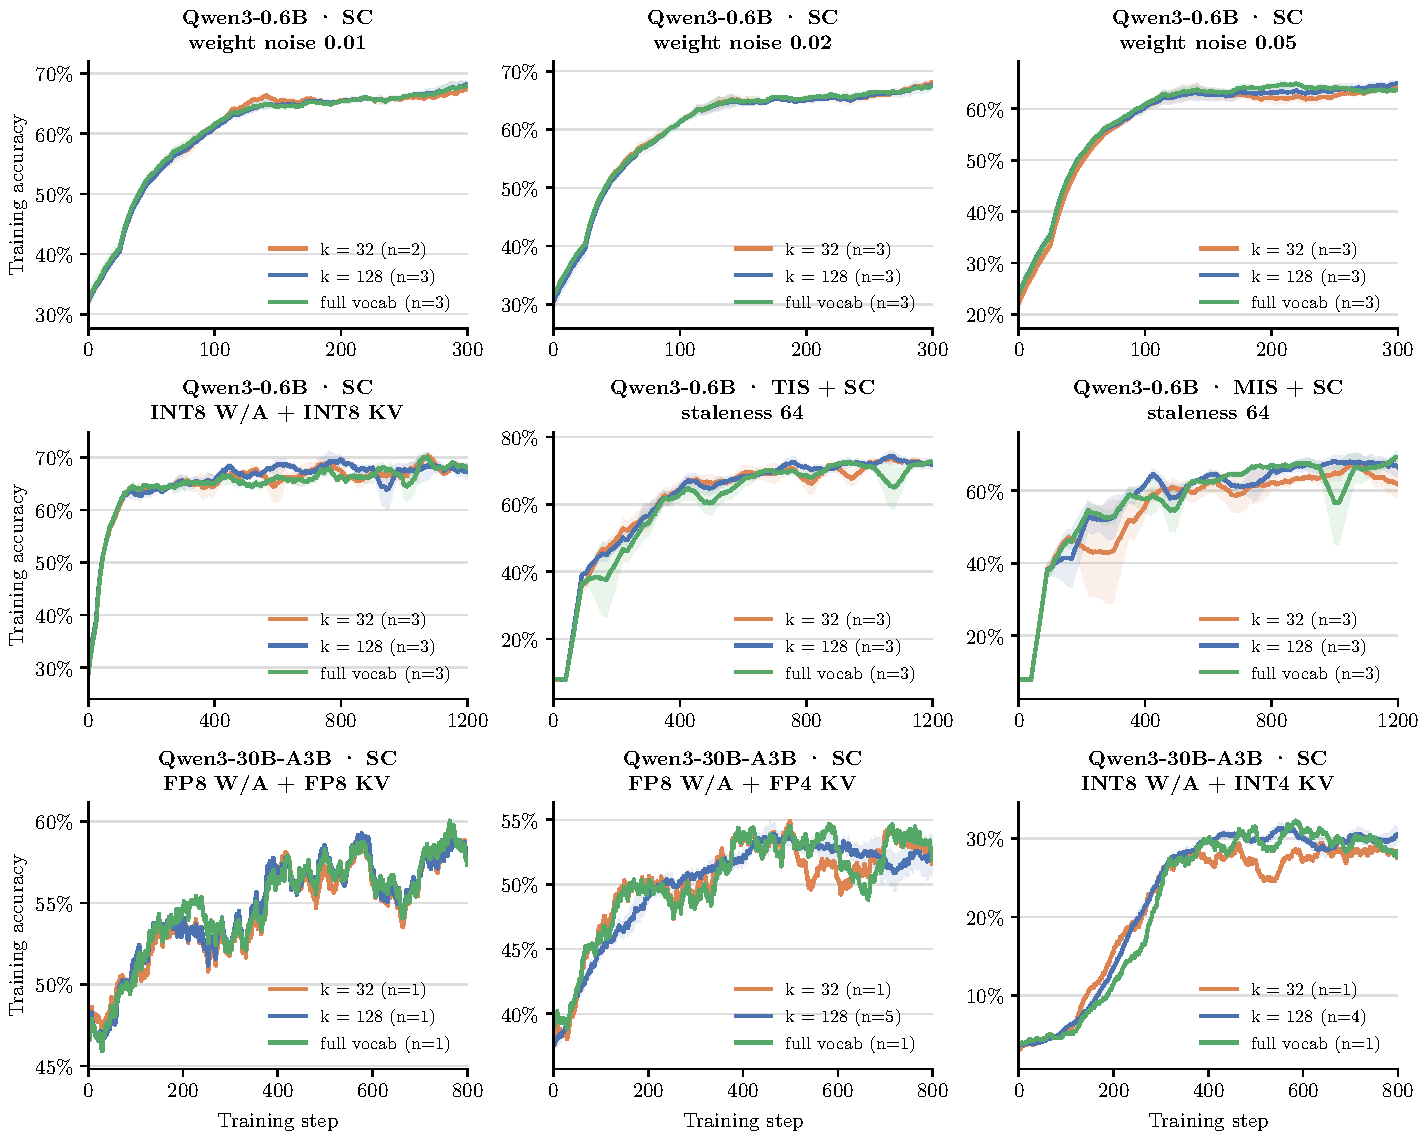
\includegraphics[width=1\linewidth]{plots/topk.pdf}
    \caption{Top-$k$  得分中心化消融实验。在所有测试情景中，使用 $k=128$  或 $k=32$  采样器的对数概率与 \Cref{eq:tail_model}  的尾部模型进行得分中心化，其效果与全词表得分中心化相当。每条曲线对应的种子数量显示在图例中。}
    \label{fig:top_k}
\end{figure}
